\chapter{Resultados}
\label{chapter:resultados}

\chapquote{¡Los números Mason! ¿Qué significan?}{Jason Hudson}

En este capítulo se muestran y detallan tanto los resultados obtenidos como los obstáculos identificado tras la implementación del sistema propuesto.

\section{Verificación y validación de los requisitos}

    En esta Sección se detalla la verificación y validación de los requisitos planteados en el Capítulo \ref{chapter:analisis}. En particular, las Tablas \ref{tabla:verificacion:requisitos_usuario}, \ref{tabla:verificacion:requisitos_funcionales} y \ref{tabla:verificacion:requisitos_no_funcionales} recogerán la verificación y validación de los requisitos de usuario, funcionales y no funcionales, respectivamente.

    \begin{xltabular}{\textwidth}{|c|c|X|c|}

        \hline
        \textbf{Requisito} & \textbf{Componente} & \textbf{Comentarios} & \textbf{¿OK?} \\
        \hline
        \endfirsthead
        
        \hline
        \textbf{Requisito} & \textbf{Componente} & \textbf{Comentarios} & \textbf{¿OK?} \\
        \hline
        \endhead
        
        \multicolumn{4}{|r|}{\textit{Continúa en la siguiente página}} \\
        \hline
        \endfoot

        \hline
        \caption{Verificación y validación de los requisitos de usuario}
        \label{tabla:verificacion:requisitos_usuario} \\
        \endlastfoot
        
        \ref{req:usuario:seguimiento_estres} & Aplicación & Implementado, mejoras planteadas & \textcolor{green}{\textbf{SI}} \\
        \hline
        \ref{req:usuario:seguimiento_depresion} & Aplicación & Implementado, mejoras planteadas & \textcolor{green}{\textbf{SI}} \\
        \hline
        \ref{req:usuario:seguimiento_soledad} & Aplicación & Implementado, mejoras planteadas & \textcolor{green}{\textbf{SI}} \\
        \hline
        \ref{req:usuario:seguimiento_suicidio} & Aplicación & Implementado, mejoras planteadas & \textcolor{green}{\textbf{SI}} \\
        \hline
        \ref{req:usuario:visualizar_estres} & Aplicación & Implementado completamente & \textcolor{green}{\textbf{SI}} \\
        \hline
        \ref{req:usuario:visualizar_depresion} & Aplicación & Implementado completamente & \textcolor{green}{\textbf{SI}} \\
        \hline
        \ref{req:usuario:visualizar_soledad} & Aplicación & Implementado completamente & \textcolor{green}{\textbf{SI}} \\
        \hline
        \ref{req:usuario:consejo_estres} & Aplicación & Implementado, mejoras planteadas & \textcolor{green}{\textbf{SI}} \\
        \hline
        \ref{req:usuario:consejo_depresion} & Aplicación & Implementado, mejoras planteadas & \textcolor{green}{\textbf{SI}} \\
        \hline
        \ref{req:usuario:consejo_soledad} & Aplicación & Implementado, mejoras planteadas & \textcolor{green}{\textbf{SI}} \\
        \hline
        \ref{req:usuario:consejo_suicidio} & Aplicación & Implementado, mejoras planteadas & \textcolor{green}{\textbf{SI}} \\
        \hline
        \ref{req:usuario:evolucion_estres} & Aplicación & Implementado completamente & \textcolor{green}{\textbf{SI}} \\
        \hline
        \ref{req:usuario:evolucion_depresion} & Aplicación & Implementado completamente & \textcolor{green}{\textbf{SI}} \\
        \hline
        \ref{req:usuario:evolucion_soledad} & Aplicación & Implementado completamente & \textcolor{green}{\textbf{SI}} \\
        \hline
        \ref{req:usuario:comunidad_estres} & Aplicación y servidor & Implementado completamente & \textcolor{green}{\textbf{SI}} \\
        \hline
        \ref{req:usuario:comunidad_depresion} & Aplicación y servidor & Implementado completamente & \textcolor{green}{\textbf{SI}} \\
        \hline
        \ref{req:usuario:comunidad_soledad} & Aplicación y servidor & Implementado completamente & \textcolor{green}{\textbf{SI}} \\
        \hline
        \ref{req:usuario:visualizar_actividad_fisica} & Aplicación & Implementado completamente & \textcolor{green}{\textbf{SI}} \\
        \hline
        \ref{req:usuario:analista_estres} & Servidor y aplicación & Implementado completamente & \textcolor{green}{\textbf{SI}} \\
        \hline
        \ref{req:usuario:analista_depresion} & Servidor y aplicación & Implementado completamente & \textcolor{green}{\textbf{SI}} \\
        \hline
        \ref{req:usuario:analista_soledad} & Servidor y aplicación & Implementado completamente & \textcolor{green}{\textbf{SI}} \\
        \hline
        \ref{req:usuario:analista_suicidio} & Servidor y aplicación & Implementado completamente & \textcolor{green}{\textbf{SI}} \\
        \hline
        \ref{req:usuario:analista_contraste} & Servidor y aplicación & Implementado completamente & \textcolor{green}{\textbf{SI}} \\
        \hline
        \ref{req:usuario:analista_actividad_fisica} & Servidor y aplicación & Implementado completamente & \textcolor{green}{\textbf{SI}} \\
    \end{xltabular}

    \begin{xltabular}{\textwidth}{|c|c|X|c|}

        \hline
        \textbf{Requisito} & \textbf{Componente} & \textbf{Comentarios} & \textbf{¿OK?} \\
        \hline
        \endfirsthead
        
        \hline
        \textbf{Requisito} & \textbf{Componente} & \textbf{Comentarios} & \textbf{¿OK?} \\
        \hline
        \endhead
        
        \multicolumn{4}{|r|}{\textit{Continúa en la siguiente página}} \\
        \hline
        \endfoot

        \hline
        \caption{Verificación y validación de los requisitos funcionales}
        \label{tabla:verificacion:requisitos_funcionales} \\
        \endlastfoot

        \ref{req:funcionales:estres_diario_info} & Aplicación & Implementado & \textcolor{green}{\textbf{SI}} \\
        \hline
        \ref{req:funcionales:estres_diario_manana} & Aplicación & Implementado junto a \ref{req:funcionales:depresion_diario_manana}, \ref{req:funcionales:soledad_diario_manana} y \ref{req:funcionales:suicidio_diario_manana}; fiabilidad variable según dispositivo (ver problema \ref{resultados:problemas:planificador}, Sección \ref{section:problemas}) & \textcolor{green}{\textbf{SI}} \\
        \hline
        \ref{req:funcionales:estres_diario_noche} & Aplicación & Implementado junto a \ref{req:funcionales:depresion_diario_noche}, \ref{req:funcionales:soledad_diario_noche},  \ref{req:funcionales:suicidio_diario_noche} y \ref{req:funcionales:contraste_diario_noche}; fiabilidad variable según dispositivo (ver problema \ref{resultados:problemas:planificador}, Sección \ref{section:problemas}) & \textcolor{green}{\textbf{SI}} \\
        \hline
        \ref{req:funcionales:estres_puntual} & Aplicación & Implementado junto a \ref{req:funcionales:depresion_puntual} y \ref{req:funcionales:soledad_puntual}; fiabilidad variable según dispositivo (ver problema \ref{resultados:problemas:planificador}, Sección \ref{section:problemas}) & \textcolor{green}{\textbf{SI}} \\
        \hline
        \ref{req:funcionales:estres_umbrales} & Aplicación & Implementado & \textcolor{green}{\textbf{SI}} \\
        \hline
        \ref{req:funcionales:estres_umbrales_consejo} & Aplicación & Implementado & \textcolor{green}{\textbf{SI}} \\
        \hline
        \ref{req:funcionales:estres_notificacion} & Aplicación & Implementado junto a \ref{req:funcionales:depresion_notificacion}, \ref{req:funcionales:soledad_notificacion}, \ref{req:funcionales:suicidio_notificacion} y \ref{req:funcionales:contraste_notificacion}; visibilidad según el permiso del usuario & \textcolor{green}{\textbf{SI}} \\
        \hline
        \ref{req:funcionales:estres_cuestionario_aplazar} & Aplicación & Implementado & \textcolor{green}{\textbf{SI}} \\
        \hline
        \ref{req:funcionales:estres_cuestionario_pendientes} & Aplicación & Implementado & \textcolor{green}{\textbf{SI}} \\
        \hline
        \ref{req:funcionales:estres_cuestionario_numero} & Aplicación & Implementado & \textcolor{green}{\textbf{SI}} \\
        \hline
        \ref{req:funcionales:estres_cuestionario_categoria} & Aplicación & Implementado & \textcolor{green}{\textbf{SI}} \\
        \hline
        \ref{req:funcionales:estres_cuestionario_consejo} & Aplicación & Implementado & \textcolor{green}{\textbf{SI}} \\
        \hline
        \ref{req:funcionales:depresion_diario_info} & Aplicación & Implementado & \textcolor{green}{\textbf{SI}} \\
        \hline
        \ref{req:funcionales:depresion_diario_manana} & Aplicación & Implementado junto a \ref{req:funcionales:estres_diario_manana}, \ref{req:funcionales:soledad_diario_manana} y \ref{req:funcionales:suicidio_diario_manana}; fiabilidad variable según dispositivo (ver problema \ref{resultados:problemas:planificador}, Sección \ref{section:problemas}) & \textcolor{green}{\textbf{SI}} \\
        \hline
        \ref{req:funcionales:depresion_diario_noche} & Aplicación & Implementado junto a \ref{req:funcionales:estres_diario_noche}, \ref{req:funcionales:soledad_diario_noche}, \ref{req:funcionales:suicidio_diario_noche} y \ref{req:funcionales:contraste_diario_noche}; fiabilidad variable según dispositivo (ver problema \ref{resultados:problemas:planificador}, Sección \ref{section:problemas}) & \textcolor{green}{\textbf{SI}} \\
        \hline
        \ref{req:funcionales:depresion_puntual} & Aplicación & Implementado junto a \ref{req:funcionales:estres_puntual} y \ref{req:funcionales:soledad_puntual}; fiabilidad variable según dispositivo (ver problema \ref{resultados:problemas:planificador}, Sección \ref{section:problemas}) & \textcolor{green}{\textbf{SI}} \\
        \hline
        \ref{req:funcionales:depresion_umbrales} & Aplicación & Implementado & \textcolor{green}{\textbf{SI}} \\
        \hline
        \ref{req:funcionales:depresion_umbrales_consejo} & Aplicación & Implementado & \textcolor{green}{\textbf{SI}} \\
        \hline
        \ref{req:funcionales:depresion_notificacion} & Aplicación & Implementado junto a \ref{req:funcionales:estres_notificacion}, \ref{req:funcionales:soledad_notificacion}, \ref{req:funcionales:suicidio_notificacion} y \ref{req:funcionales:contraste_notificacion}; visibilidad según el permiso del usuario & \textcolor{green}{\textbf{SI}} \\
        \hline
        \ref{req:funcionales:depresion_cuestionario_aplazar} & Aplicación & Implementado & \textcolor{green}{\textbf{SI}} \\
        \hline
        \ref{req:funcionales:depresion_cuestionario_pendientes} & Aplicación & Implementado & \textcolor{green}{\textbf{SI}} \\
        \hline
        \ref{req:funcionales:depresion_cuestionario_numero} & Aplicación & Implementado & \textcolor{green}{\textbf{SI}} \\
        \hline
        \ref{req:funcionales:depresion_cuestionario_categoria} & Aplicación & Implementado & \textcolor{green}{\textbf{SI}} \\
        \hline
        \ref{req:funcionales:depresion_cuestionario_consejo} & Aplicación & Implementado & \textcolor{green}{\textbf{SI}} \\
        \hline
        \ref{req:funcionales:soledad_diario_info} & Aplicación & Implementado & \textcolor{green}{\textbf{SI}} \\
        \hline
        \ref{req:funcionales:soledad_diario_manana} & Aplicación & Implementado junto a \ref{req:funcionales:estres_diario_manana}, \ref{req:funcionales:depresion_diario_manana} y \ref{req:funcionales:suicidio_diario_manana}; fiabilidad variable según dispositivo (ver problema \ref{resultados:problemas:planificador}, Sección \ref{section:problemas}) & \textcolor{green}{\textbf{SI}} \\
        \hline
        \ref{req:funcionales:soledad_diario_noche} & Aplicación & Implementado junto a \ref{req:funcionales:estres_diario_noche}, \ref{req:funcionales:depresion_diario_noche},  \ref{req:funcionales:suicidio_diario_noche} y \ref{req:funcionales:contraste_diario_noche}; fiabilidad variable según dispositivo (ver problema \ref{resultados:problemas:planificador}, Sección \ref{section:problemas}) & \textcolor{green}{\textbf{SI}} \\
        \hline
        \ref{req:funcionales:soledad_puntual} & Aplicación & Implementado junto a \ref{req:funcionales:estres_puntual}, y \ref{req:funcionales:depresion_puntual}; fiabilidad variable según dispositivo (ver problema \ref{resultados:problemas:planificador}, Sección \ref{section:problemas}) & \textcolor{green}{\textbf{SI}} \\
        \hline
        \ref{req:funcionales:soledad_umbrales} & Aplicación & Implementado & \textcolor{green}{\textbf{SI}} \\
        \hline
        \ref{req:funcionales:soledad_umbrales_consejo} & Aplicación & Implementado & \textcolor{green}{\textbf{SI}} \\
        \hline
        \ref{req:funcionales:soledad_notificacion} & Aplicación & Implementado junto a \ref{req:funcionales:estres_notificacion}, \ref{req:funcionales:depresion_notificacion}, \ref{req:funcionales:suicidio_notificacion} y \ref{req:funcionales:contraste_notificacion}; visibilidad según el permiso del usuario & \textcolor{green}{\textbf{SI}} \\
        \hline
        \ref{req:funcionales:soledad_cuestionario_aplazar} & Aplicación & Implementado & \textcolor{green}{\textbf{SI}} \\
        \hline
        \ref{req:funcionales:soledad_cuestionario_pendientes} & Aplicación & Implementado & \textcolor{green}{\textbf{SI}} \\
        \hline
        \ref{req:funcionales:soledad_cuestionario_numero} & Aplicación & Implementado & \textcolor{green}{\textbf{SI}} \\
        \hline
        \ref{req:funcionales:soledad_cuestionario_categoria} & Aplicación & Implementado & \textcolor{green}{\textbf{SI}} \\
        \hline
        \ref{req:funcionales:soledad_cuestionario_consejo} & Aplicación & Implementado & \textcolor{green}{\textbf{SI}} \\
        \hline
        \ref{req:funcionales:suicidio_diario_info} & Aplicación & Implementado & \textcolor{green}{\textbf{SI}} \\
        \hline
        \ref{req:funcionales:suicidio_diario_manana} & Aplicación & Implementado junto a \ref{req:funcionales:estres_diario_manana}, \ref{req:funcionales:depresion_diario_manana} y \ref{req:funcionales:soledad_diario_manana}; fiabilidad variable según dispositivo (ver problema \ref{resultados:problemas:planificador}, Sección \ref{section:problemas}) & \textcolor{green}{\textbf{SI}} \\
        \hline
        \ref{req:funcionales:suicidio_diario_noche} & Aplicación & Implementado junto a \ref{req:funcionales:estres_diario_noche}, \ref{req:funcionales:depresion_diario_noche},  \ref{req:funcionales:soledad_diario_noche} y \ref{req:funcionales:contraste_diario_noche}; fiabilidad variable según dispositivo (ver problema \ref{resultados:problemas:planificador}, Sección \ref{section:problemas}) & \textcolor{green}{\textbf{SI}} \\
        \hline
        \ref{req:funcionales:suicidio_umbrales} & Aplicación & Implementado & \textcolor{green}{\textbf{SI}} \\
        \hline
        \ref{req:funcionales:suicidio_consejo} & Aplicación & Implementado & \textcolor{green}{\textbf{SI}} \\
        \hline
        \ref{req:funcionales:suicidio_notificacion} & Aplicación & Implementado junto a \ref{req:funcionales:estres_notificacion}, \ref{req:funcionales:depresion_notificacion}, \ref{req:funcionales:soledad_notificacion} y \ref{req:funcionales:contraste_notificacion}; visibilidad según el permiso del usuario & \textcolor{green}{\textbf{SI}} \\
        \hline
        \ref{req:funcionales:suicidio_cuestionario_aplazar} & Aplicación & Implementado & \textcolor{green}{\textbf{SI}} \\
        \hline
        \ref{req:funcionales:suicidio_cuestionario_pendientes} & Aplicación & Implementado & \textcolor{green}{\textbf{SI}} \\
        \hline
        \ref{req:funcionales:suicidio_cuestionario_consejo} & Aplicación & Implementado & \textcolor{green}{\textbf{SI}} \\
        \hline
        \ref{req:funcionales:visualizar_estres_numero} & Aplicación & Implementado & \textcolor{green}{\textbf{SI}} \\
        \hline
        \ref{req:funcionales:visualizar_estres_categoria} & Aplicación & Implementado & \textcolor{green}{\textbf{SI}} \\
        \hline
        \ref{req:funcionales:visualizar_depresion_numero} & Aplicación & Implementado & \textcolor{green}{\textbf{SI}} \\
        \hline
        \ref{req:funcionales:visualizar_depresion_categoria} & Aplicación & Implementado & \textcolor{green}{\textbf{SI}} \\
        \hline
        \ref{req:funcionales:visualizar_soledad_numero} & Aplicación & Implementado & \textcolor{green}{\textbf{SI}} \\
        \hline
        \ref{req:funcionales:visualizar_soledad_categoria} & Aplicación & Implementado & \textcolor{green}{\textbf{SI}} \\
        \hline
        \ref{req:funcionales:consejo_cuestionario_estres} & Aplicación & Implementado & \textcolor{green}{\textbf{SI}} \\
        \hline
        \ref{req:funcionales:consejo_visualizacion_estres} & Aplicación & Implementado & \textcolor{green}{\textbf{SI}} \\
        \hline
        \ref{req:funcionales:consejo_cuestionario_depresion} & Aplicación & Implementado & \textcolor{green}{\textbf{SI}} \\
        \hline
        \ref{req:funcionales:consejo_visualizacion_depresion} & Aplicación & Implementado & \textcolor{green}{\textbf{SI}} \\
        \hline
        \ref{req:funcionales:consejo_cuestionario_soledad} & Aplicación & Implementado & \textcolor{green}{\textbf{SI}} \\
        \hline
        \ref{req:funcionales:consejo_visualizacion_soledad} & Aplicación & Implementado & \textcolor{green}{\textbf{SI}} \\
        \hline
        \ref{req:funcionales:consejo_cuestionario_suicidio} & Aplicación & Implementado & \textcolor{green}{\textbf{SI}} \\
        \hline
        \ref{req:funcionales:evolucion_estres_dia} & Aplicación & Implementado & \textcolor{green}{\textbf{SI}} \\
        \hline
        \ref{req:funcionales:evolucion_estres_semana} & Aplicación & Implementado & \textcolor{green}{\textbf{SI}} \\
        \hline
        \ref{req:funcionales:evolucion_estres_mes} & Aplicación & Implementado & \textcolor{green}{\textbf{SI}} \\
        \hline
        \ref{req:funcionales:evolucion_estres_elegir} & Aplicación & Implementado & \textcolor{green}{\textbf{SI}} \\
        \hline
        \ref{req:funcionales:evolucion_depresion_dia} & Aplicación & Implementado & \textcolor{green}{\textbf{SI}} \\
        \hline
        \ref{req:funcionales:evolucion_depresion_semana} & Aplicación & Implementado & \textcolor{green}{\textbf{SI}} \\
        \hline
        \ref{req:funcionales:evolucion_depresion_mes} & Aplicación & Implementado & \textcolor{green}{\textbf{SI}} \\
        \hline
        \ref{req:funcionales:evolucion_depresion_elegir} & Aplicación & Implementado & \textcolor{green}{\textbf{SI}} \\
        \hline
        \ref{req:funcionales:evolucion_soledad_dia} & Aplicación & Implementado & \textcolor{green}{\textbf{SI}} \\
        \hline
        \ref{req:funcionales:evolucion_soledad_semana} & Aplicación & Implementado & \textcolor{green}{\textbf{SI}} \\
        \hline
        \ref{req:funcionales:evolucion_soledad_mes} & Aplicación & Implementado & \textcolor{green}{\textbf{SI}} \\
        \hline
        \ref{req:funcionales:evolucion_soledad_elegir} & Aplicación & Implementado & \textcolor{green}{\textbf{SI}} \\
        \hline
        \ref{req:funcionales:comunidad_estres_dia_anterior_ver} & Aplicación & Implementado & \textcolor{green}{\textbf{SI}} \\
        \hline
        \ref{req:funcionales:comunidad_estres_siete_dias_ver} & Aplicación & Implementado & \textcolor{green}{\textbf{SI}} \\
        \hline
        \ref{req:funcionales:comunidad_estres_semana_actual_ver} & Aplicación & Implementado & \textcolor{green}{\textbf{SI}} \\
        \hline
        \ref{req:funcionales:comunidad_depresion_dia_anterior_ver} & Aplicación & Implementado & \textcolor{green}{\textbf{SI}} \\
        \hline
        \ref{req:funcionales:comunidad_depresion_siete_dias_ver} & Aplicación & Implementado & \textcolor{green}{\textbf{SI}} \\
        \hline
        \ref{req:funcionales:comunidad_depresion_semana_actual_ver} & Aplicación & Implementado & \textcolor{green}{\textbf{SI}} \\
        \hline
        \ref{req:funcionales:comunidad_soledad_dia_anterior_ver} & Aplicación & Implementado & \textcolor{green}{\textbf{SI}} \\
        \hline
        \ref{req:funcionales:comunidad_soledad_siete_dias_ver} & Aplicación & Implementado & \textcolor{green}{\textbf{SI}} \\
        \hline
        \ref{req:funcionales:comunidad_soledad_semana_actual_ver} & Aplicación & Implementado & \textcolor{green}{\textbf{SI}} \\
        \hline
        \ref{req:funcionales:permiso_distancia} & Aplicación & Implementado & \textcolor{green}{\textbf{SI}} \\
        \hline
        \ref{req:funcionales:permiso_desnivel} & Aplicación & Implementado & \textcolor{green}{\textbf{SI}} \\
        \hline
        \ref{req:funcionales:permiso_ejercicio} & Aplicación & Implementado & \textcolor{green}{\textbf{SI}} \\
        \hline
        \ref{req:funcionales:permiso_plantas} & Aplicación & Implementado & \textcolor{green}{\textbf{SI}} \\
        \hline
        \ref{req:funcionales:permiso_pulsaciones} & Aplicación & Implementado & \textcolor{green}{\textbf{SI}} \\
        \hline
        \ref{req:funcionales:permiso_sueno} & Aplicación & Implementado & \textcolor{green}{\textbf{SI}} \\
        \hline
        \ref{req:funcionales:permiso_pasos} & Aplicación & Implementado & \textcolor{green}{\textbf{SI}} \\
        \hline
        \ref{req:funcionales:permiso_calorias} & Aplicación & Implementado & \textcolor{green}{\textbf{SI}} \\
        \hline
        \ref{req:funcionales:permiso_peso} & Aplicación & Implementado & \textcolor{green}{\textbf{SI}} \\
        \hline
        \ref{req:funcionales:extraer_distancia} & Aplicación, \gls{wearable} & Implementado indirectamente, a través de la lectura de los datos extraídos por \textit{Salud Conectada} & \textcolor{green}{\textbf{SI}} \\
        \hline
        \ref{req:funcionales:extraer_desnivel} & Aplicación, \gls{wearable} & Implementado indirectamente, a través de la lectura de los datos extraídos por \textit{Salud Conectada} & \textcolor{green}{\textbf{SI}} \\
        \hline
        \ref{req:funcionales:extraer_ejercicio} & Aplicación, \gls{wearable} & Implementado indirectamente, a través de la lectura de los datos extraídos por \textit{Salud Conectada} & \textcolor{green}{\textbf{SI}} \\
        \hline
        \ref{req:funcionales:extraer_plantas} & Aplicación, \gls{wearable} & Implementado indirectamente, a través de la lectura de los datos extraídos por \textit{Salud Conectada} & \textcolor{green}{\textbf{SI}} \\
        \hline
        \ref{req:funcionales:extraer_pulsaciones} & Aplicación, \gls{wearable} & Implementado indirectamente, a través de la lectura de los datos extraídos por \textit{Salud Conectada} & \textcolor{green}{\textbf{SI}} \\
        \hline
        \ref{req:funcionales:extraer_sueno} & Aplicación, \gls{wearable} & Implementado indirectamente, a través de la lectura de los datos extraídos por \textit{Salud Conectada} & \textcolor{green}{\textbf{SI}} \\
        \hline
        \ref{req:funcionales:extraer_pasos} & Aplicación, \gls{wearable} & Implementado indirectamente, a través de la lectura de los datos extraídos por \textit{Salud Conectada} & \textcolor{green}{\textbf{SI}} \\
        \hline
        \ref{req:funcionales:extraer_calorias} & Aplicación, \gls{wearable} & Implementado indirectamente, a través de la lectura de los datos extraídos por \textit{Salud Conectada} & \textcolor{green}{\textbf{SI}} \\
        \hline
        \ref{req:funcionales:extraer_peso} & Aplicación, \gls{wearable} & Implementado indirectamente, a través de la lectura de los datos extraídos por \textit{Salud Conectada} & \textcolor{green}{\textbf{SI}} \\
        \hline
        \ref{req:funcionales:visualizar_distancia} & Aplicación & Implementado & \textcolor{green}{\textbf{SI}} \\
        \hline
        \ref{req:funcionales:visualizar_desnivel} & Aplicación & Implementado & \textcolor{green}{\textbf{SI}} \\
        \hline
        \ref{req:funcionales:visualizar_ejercicio} & Aplicación & Implementado & \textcolor{green}{\textbf{SI}} \\
        \hline
        \ref{req:funcionales:visualizar_plantas} & Aplicación & Implementado & \textcolor{green}{\textbf{SI}} \\
        \hline
        \ref{req:funcionales:visualizar_frecuencia} & Aplicación & Implementado & \textcolor{green}{\textbf{SI}} \\
        \hline
        \ref{req:funcionales:visualizar_sueno} & Aplicación & Implementado & \textcolor{green}{\textbf{SI}} \\
        \hline
        \ref{req:funcionales:visualizar_pasos} & Aplicación & Implementado & \textcolor{green}{\textbf{SI}} \\
        \hline
        \ref{req:funcionales:visualizar_calorias} & Aplicación & Implementado & \textcolor{green}{\textbf{SI}} \\
        \hline
        \ref{req:funcionales:visualizar_peso} & Aplicación & Implementado & \textcolor{green}{\textbf{SI}} \\
        \hline
        \ref{req:funcionales:estres_diario_formato} & Servidor & Implementado & \textcolor{green}{\textbf{SI}} \\
        \hline
        \ref{req:funcionales:estres_puntual_formato} & Servidor & Implementado & \textcolor{green}{\textbf{SI}} \\
        \hline
        \ref{req:funcionales:estres_finalizado_servidor} & Servidor, aplicación & Implementado & \textcolor{green}{\textbf{SI}} \\
        \hline
        \ref{req:funcionales:depresion_diario_formato} & Servidor & Implementado & \textcolor{green}{\textbf{SI}} \\
        \hline
        \ref{req:funcionales:depresion_puntual_formato} & Servidor & Implementado & \textcolor{green}{\textbf{SI}} \\
        \hline
        \ref{req:funcionales:depresion_finalizado_servidor} & Servidor, aplicación & Implementado & \textcolor{green}{\textbf{SI}} \\
        \hline
        \ref{req:funcionales:soledad_diario_formato} & Servidor & Implementado & \textcolor{green}{\textbf{SI}} \\
        \hline
        \ref{req:funcionales:soledad_puntual_formato} & Servidor & Implementado & \textcolor{green}{\textbf{SI}} \\
        \hline
        \ref{req:funcionales:soledad_finalizado_servidor} & Servidor, aplicación & Implementado & \textcolor{green}{\textbf{SI}} \\
        \hline
        \ref{req:funcionales:suicidio_diario_formato} & Servidor & Implementado & \textcolor{green}{\textbf{SI}} \\
        \hline
        \ref{req:funcionales:suicidio_finalizado_servidor} & Servidor, aplicación & Implementado & \textcolor{green}{\textbf{SI}} \\
        \hline
        \ref{req:funcionales:contraste_diario_info} & Aplicación & Implementado & \textcolor{green}{\textbf{SI}} \\
        \hline
        \ref{req:funcionales:contraste_diario_noche} & Aplicación & Implementado junto a \ref{req:funcionales:estres_diario_noche},
        \ref{req:funcionales:depresion_diario_noche}, \ref{req:funcionales:soledad_diario_noche} y   \ref{req:funcionales:suicidio_diario_noche}; fiabilidad variable según dispositivo (ver problema \ref{resultados:problemas:planificador}, Sección \ref{section:problemas}) & \textcolor{green}{\textbf{SI}} \\
        \hline
        \ref{req:funcionales:contraste_notificacion} & Aplicación & Implementado junto a \ref{req:funcionales:estres_notificacion}, \ref{req:funcionales:depresion_notificacion}, \ref{req:funcionales:soledad_notificacion} y \ref{req:funcionales:suicidio_notificacion}; visibilidad según el permiso del usuario & \textcolor{green}{\textbf{SI}} \\
        \hline
        \ref{req:funcionales:contraste_cuestionario_aplazar} & Aplicación, aplicación & Implementado & \textcolor{green}{\textbf{SI}} \\
        \hline
        \ref{req:funcionales:contraste_cuestionario_pendientes} & Aplicación, aplicación & Implementado & \textcolor{green}{\textbf{SI}} \\
        \hline
        \ref{req:funcionales:contraste_diario_formato} & Servidor & Implementado & \textcolor{green}{\textbf{SI}} \\
        \hline
        \ref{req:funcionales:contraste_finalizado_servidor} & Servidor, aplicación & Implementado & \textcolor{green}{\textbf{SI}} \\
        \hline
        \ref{req:funcionales:actividad_fisica_recoger} & Servidor, aplicación & Implementado & \textcolor{green}{\textbf{SI}} \\
        \hline
        \ref{req:funcionales:distancia_formato} & Servidor & Implementado & \textcolor{green}{\textbf{SI}} \\
        \hline
        \ref{req:funcionales:desnivel_formato} & Servidor & Implementado & \textcolor{green}{\textbf{SI}} \\
        \hline
        \ref{req:funcionales:ejercicio_formato} & Servidor & Implementado & \textcolor{green}{\textbf{SI}} \\
        \hline
        \ref{req:funcionales:plantas_formato} & Servidor & Implementado & \textcolor{green}{\textbf{SI}} \\
        \hline
        \ref{req:funcionales:frecuencia_formato} & Servidor & Implementado & \textcolor{green}{\textbf{SI}} \\
        \hline
        \ref{req:funcionales:sueno_formato} & Servidor & Implementado & \textcolor{green}{\textbf{SI}} \\
        \hline
        \ref{req:funcionales:pasos_formato} & Servidor & Implementado & \textcolor{green}{\textbf{SI}} \\
        \hline
        \ref{req:funcionales:calorias_formato} & Servidor & Implementado & \textcolor{green}{\textbf{SI}} \\
        \hline
        \ref{req:funcionales:peso_formato} & Servidor & Implementado & \textcolor{green}{\textbf{SI}} \\
    \end{xltabular}

    \begin{xltabular}{\textwidth}{|c|c|X|c|}

        \hline
        \textbf{Requisito} & \textbf{Componente} & \textbf{Comentarios} & \textbf{¿OK?} \\
        \hline
        \endfirsthead
        
        \hline
        \textbf{Requisito} & \textbf{Componente} & \textbf{Comentarios} & \textbf{¿OK?} \\
        \hline
        \endhead
        
        \multicolumn{4}{|r|}{\textit{Continúa en la siguiente página}} \\
        \hline
        \endfoot

        \hline
        \caption{Verificación y validación de los requisitos no funcionales}
        \label{tabla:verificacion:requisitos_no_funcionales} \\
        \endlastfoot
        
        \ref{req:no_funcionales:envio_internet} & Aplicación & Implementado & \textcolor{green}{\textbf{SI}} \\
        \hline
        \ref{req:no_funcionales:envio_aplazar} & Aplicación & Implementado & \textcolor{green}{\textbf{SI}} \\
        \hline
        \ref{req:no_funcionales:envio_solo_ultimos} & Aplicación & Implementado & \textcolor{green}{\textbf{SI}} \\
        \hline
        \ref{req:no_funcionales:nuevas_versiones_android} & Aplicación & Considerado en diseño e implementación; no implementable directamente & \textcolor{green}{\textbf{SI}} \\
        \hline
        \ref{req:no_funcionales:nuevas_categorias_fisicas} & Aplicación & Considerado en diseño e implementación; no implementable directamente & \textcolor{green}{\textbf{SI}} \\
        \hline
        \ref{req:no_funcionales:solid} & Transversal & Principios seguidos en la implementación, no implementable directamente & \textcolor{green}{\textbf{SI}} \\
        \hline
        \ref{req:no_funcionales:notificacion_salud_conectada} & Aplicación & Implementado & \textcolor{green}{\textbf{SI}} \\
        \hline
        \ref{req:no_funcionales:frecuencia_subida_fisica} & Aplicación & Implementado, fiabilidad variable según dispositivo (ver problema \ref{resultados:problemas:planificador}) & \textcolor{green}{\textbf{SI}} \\
        \hline
        \ref{req:no_funcionales:frecuencia_subida_diarios} & Aplicación & Implementado, fiabilidad variable según dispositivo (ver problema \ref{resultados:problemas:planificador}) & \textcolor{green}{\textbf{SI}} \\
        \hline
        \ref{req:no_funcionales:frecuencia_subida_puntuales} & Aplicación & Implementado, fiabilidad variable según dispositivo (ver problema \ref{resultados:problemas:planificador}) & \textcolor{green}{\textbf{SI}} \\
        \hline
        \ref{req:no_funcionales:guardar_ultima_subida} & Aplicación & Implementado & \textcolor{green}{\textbf{SI}} \\
        \hline
        \ref{req:no_funcionales:version_android} & Aplicación & Implementado & \textcolor{green}{\textbf{SI}} \\
        \hline
        \ref{req:no_funcionales:soporte_wearable} & Aplicación, \gls{wearable} & Garantizado por \textit{Salud Conectada} & \textcolor{green}{\textbf{SI}} \\
        \hline
        \ref{req:no_funcionales:id_anonimo} & Aplicación & Implementado & \textcolor{green}{\textbf{SI}} \\
        \hline
        \ref{req:no_funcionales:cifrado_bd} & Aplicación & Implementado & \textcolor{green}{\textbf{SI}} \\
        \hline
        \ref{req:no_funcionales:inmutabilidad} & Aplicación & Implementado & \textcolor{green}{\textbf{SI}} \\
        \hline
        \ref{req:no_funcionales:datos_solo_cientificos} & Servidor & Planteado como línea futura & \textcolor{red}{\textbf{NO}} \\
        \hline
        \ref{req:no_funcionales:ddos} & Servidor & Planteado como línea futura & \textcolor{red}{\textbf{NO}} \\
        \hline
        \ref{req:no_funcionales:cifrado_comunicaciones} & Aplicación, servidor & Planteado como línea futura & \textcolor{red}{\textbf{NO}} \\
        \hline
        \ref{req:no_funcionales:politica_privacidad} & Transversal & Planteado como línea futura & \textcolor{red}{\textbf{NO}} \\
        \hline
        \ref{req:no_funcionales:ui_responsive} & Aplicación & Implementado & \textcolor{green}{\textbf{SI}} \\
        \hline
        \ref{req:no_funcionales:ui_tamanio_pantalla} & Aplicación & Implementado & \textcolor{green}{\textbf{SI}} \\
        \hline
        \ref{req:no_funcionales:ui_orientacion_soporte} & Aplicación & Implementado & \textcolor{green}{\textbf{SI}} \\
        \hline
        \ref{req:no_funcionales:ui_orientacion_dinamica} & Aplicación & Garantizado por defecto por Android & \textcolor{green}{\textbf{SI}} \\
        \hline
        \ref{req:no_funcionales:bienvenida} & Aplicación & Implementado & \textcolor{green}{\textbf{SI}} \\
        \hline
        \ref{req:no_funcionales:bienvenida_demanda} & Aplicación & Implementado & \textcolor{green}{\textbf{SI}} \\
        \hline
        \ref{req:no_funcionales:contraste} & Aplicación & Garantizado por \textit{Material Design Builder} \cite{material_design_material_nodate-1} & \textcolor{green}{\textbf{SI}} \\
        \hline
        \ref{req:no_funcionales:colores_tranquilidad} & Aplicación & Implementado & \textcolor{green}{\textbf{SI}} \\
        \hline
        \ref{req:no_funcionales:modo_claro_oscuro} & Aplicación & Garantizado por \textit{Material Design Builder} \cite{material_design_material_nodate-1} & \textcolor{green}{\textbf{SI}} \\
        \hline
        \ref{req:no_funcionales:modo_defecto} & Aplicación & Garantizado por defecto por Android & \textcolor{green}{\textbf{SI}} \\
        \hline
        \ref{req:no_funcionales:modo_demanda} & Aplicación & Implementado & \textcolor{green}{\textbf{SI}} \\
        \hline
        \ref{req:no_funcionales:colores_dinamico} & Aplicación & Garantizado por defecto por Android & \textcolor{green}{\textbf{SI}} \\
        \hline
        \ref{req:no_funcionales:idioma_espanol} & Aplicación & Implementado & \textcolor{green}{\textbf{SI}} \\
        \hline
        \ref{req:no_funcionales:idioma_ingles} & Aplicación & Implementado & \textcolor{green}{\textbf{SI}} \\
        \hline
        \ref{req:no_funcionales:idioma_defecto} & Aplicación & Garantizado por defecto por Android & \textcolor{green}{\textbf{SI}} \\
        \hline
    \end{xltabular}

\section{Problemas encontrados}
    \label{section:problemas}

    A lo largo de esta sección serán detallados los problemas encontrados durante el desarrollo de este \gls{tfm}. A continuación, se listarán y describirán cada uno de ellos.
    
    \begin{enumerate}
        \item \textbf{Falta de experiencia del autor en la \gls{iss}}: el autor es plenamente consciente de la dificultad de la elaboración de los planes de estudios para cubrir todas las áreas relevantes de conocimiento, pero quiere poner de manifiesto que la \gls{iss} solo se ha cubierto mediante dos asignaturas, una de ellas en el \textit{Doble Grado en Ingeniería de Computadores y Tecnologías para la Sociedad de la Información} y la otra en este máster.
        
        Para interiorizar plenamente los conceptos de la \gls{iss}, el autor considera que es necesaria cierta experiencia práctica; por lo que se introdujo como un objetivo fundamental de este \gls{tfm} desde el inicio. Esta casuística ha ralentizado el ritmo de realización de este proyecto, si bien ha supuesto un enorme aprendizaje para el autor.
        
        \item \textbf{Falta de experiencia del autor en el desarrollo de aplicaciones móviles}: se trata de un problema muy similar al anterior. Si bien el autor había desarrollado dos aplicaciones pequeñas en sendas asignaturas, se ha tratado del primer desarrollo a mayor escala; especialmente, en cuanto al diseño e implementación de interfaces gráficas.
    
        Esta circunstancia ha supuesto numerosos retos para el autor, tales como el aprendizaje de nuevos lenguajes de programación, el uso de patrones de diseño como inyección de dependencias o factoría o la realización de diseños \gls{responsive}. Como en el caso anterior, ha frenado el ritmo de desarrollo, pero a cambio ha supuesto una incalculable experiencia que ha permitido el aprendizaje de numerosos conceptos y/o técnicas.
    
        \item \label{resultados:problemas:planificador} \textbf{Agresivas optimizaciones de batería en algunos dispositivos}: este problema fue descubierto realizando pruebas en dispositivos reales al componente \textit{Work Manager}. En dichas comprobaciones se constató en que algunos dispositivos, como el \textit{Pocophone F1} del autor, el sistema operativo nunca ejecutaba en segundo plano las tareas planificadas, realizándose todas ellas de golpe únicamente cuando el usuario abría la aplicación.
    
        Dado que este comportamiento no está documentado oficialmente, una investigación fue realizada para tratar de descubrir el problema de fondo y buscar una solución. Al parecer se trata de un problema reportado desde al menos el año 2017 \cite{mathew_why_2017}, en el cual ciertos fabricantes de \glspl{smartphone}, tales como Xiaomi, Samsung, Oppo o Redmi, realizan modificaciones en sus versiones de Android que rompen con el cumplimiento de las \gls{api} \cite{android_public_tracker_chinese_nodate} \cite{android_public_tracker_request_nodate}
        levantando polémica ya que según las políticas de Android no está permitido \cite{cylon999_workmanager_2018}.
    
        Con la finalidad de ahorrar batería, en estas versiones el sistema cierra forzosamente ciertas aplicaciones, cancelando todas las tareas en segundo plano \cite{manohar_is_2020}. Las aplicaciones más utilizadas por los usuarios, como \textit{WhatsApp}, parecen estar en una \textit{lista blanca}, lo que genera un enorme agravio comparativo; ya que el usuario debe desactivar manualmente esta optimización de batería \cite{shukla_work_2021}.
    
        Sobre este problema se pueden encontrar iniciativas como \textit{Don't kill my app} \cite{dont_kill_my_app_our_nodate} que están arrojando visibilidad a este fenómeno, a través de charlas y de la evaluación de estas políticas según cada fabricante.
    
        \item \textbf{Escaso soporte oficial de los fabricantes de \glspl{wearable} a \textit{Salud Conectada}}: desde el anuncio de \textit{Salud Conectada}, únicamente dos fabricantes soportan dicho \gls{framework}: Samsung y la propia Fitbit (propiedad de la propia Google desde 2019). 
        
        En el caso de Samsung, se realizaron pruebas con una \textit{Samsung Galaxy Fit 2}, descubriéndose que la pulsera únicamente era capaz de escribir en \textit{Salud Conectada} datos de sueño, como se puede ver en la Figura \ref{figure:problemas:samsung_sueño}.
    
        \begin{figure}[h]
            \centering
            \includegraphics[width=0.45\textwidth]{figures/escritura_solo_sueño.jpg}
            \caption{Registro de lectura/escritura con una \textit{Samsung Galaxy Fit 2}}
            \label{figure:problemas:samsung_sueño}
        \end{figure}
    
        Estos problemas de escritura fueron reportados por la comunidad en los casos de pulsaciones \cite{jauwaadshams_heart_2023}, pasos \cite{ste1603137554_samsung_2022} o directamente, no funcionando en Android 14 \cite{muzzas_samsung_2023}.
    
        Para resolver estas cuestiones, se apostó por utilizar únicamente pulseras Fitbit para el desarrollo, pero en cualquier caso estos problemas tienen un impacto directo en el uso de otras pulseras por parte de los usuarios.
        
        \item \textbf{Inestabilidad del ecosistema \textit{Salud Conectada}}. A fecha de julio de 2024, el \gls{sdk} ofrecido por Google continúa aún en fase \textit{alpha}. Durante la realización de este \gls{tfm} se han producido numerosos cambios en dicho componente, tales como las modificaciones en las \gls{api} ofrecidas para los desarrolladores, o la necesidad de realizar una migración detallada para soportar Android 14 \cite{android_developers_migrate_nodate}, lo que ha supuesto un consumo adicional de recursos mantener la aplicación actualizada.
    
        \item \textbf{Falta de madurez y adopción de \textit{Jetpack Compose} y \textit{Material Design 3}}: se ha tratado de un problema sistemático y persistente a lo largo de todo el proyecto, que ha supuesto un sinfín de retos y de dificultades técnicas. Algunos de ellos fueron resueltos mediante el uso de librerías, como se especificó en la Sección \ref{section:implementacion:librerias_app}.
    
        En el caso de \textit{Jetpack Compose} lleva aproximadamente tres años en el mercado; aún presenta deficiencias a resolver. El caso más paradigmático encontrado en este proyecto ha sido el procedimiento de paso de parámetros en la navegación entre ventanas, el cual ha tenido que \textit{resolver} la comunidad mediante librerías como \href{https://github.com/raamcosta/compose-destinations}{\textit{Compose Destinations}}.  
        
        Por otra parte, la aún escasa adopción de este \gls{framework} ha supuesto una clara desventaja en el acceso a documentación y recursos actualizados; provocando un incremento de dificultad más que notable de tareas tan habituales como la automatización de pruebas.
    
        Un caso similar ha sucedido con \textit{Material Design 3}, con la salvedad que su primera versión estable fue lanzada en octubre de 2022; pocas semanas después del comienzo de este proyecto. La ausencia de adopción masiva es comprensible, pero no la falta de madurez de la misma. 
        
        Un caso paradigmático es el componente \textit{date picker}, utilizado para que el usuario pueda seleccionar fechas. Siete mes después de la primera versión estable se introdujo dicho componente en un estado experimental o inestable, el cual sigue sin haber abandonado casi dos años después de su especificación, como se puede ver en la Figura \ref{figure:problemas:date_picker}. Para resolver estos problemas, nuevamente la comunidad ha tomado la alternativa y ha propuesto implementaciones de acuerdo a esta especificación, como \href{https://github.com/maxkeppeler/sheets-compose-dialogs}{\textit{Sheets-Compose-Dialogs}} o añadiendo nuevos componentes, como en \href{https://github.com/alorma/Compose-Settings}{\textit{Compose Settings}}.
    
        \begin{figure}[h]
            \centering
            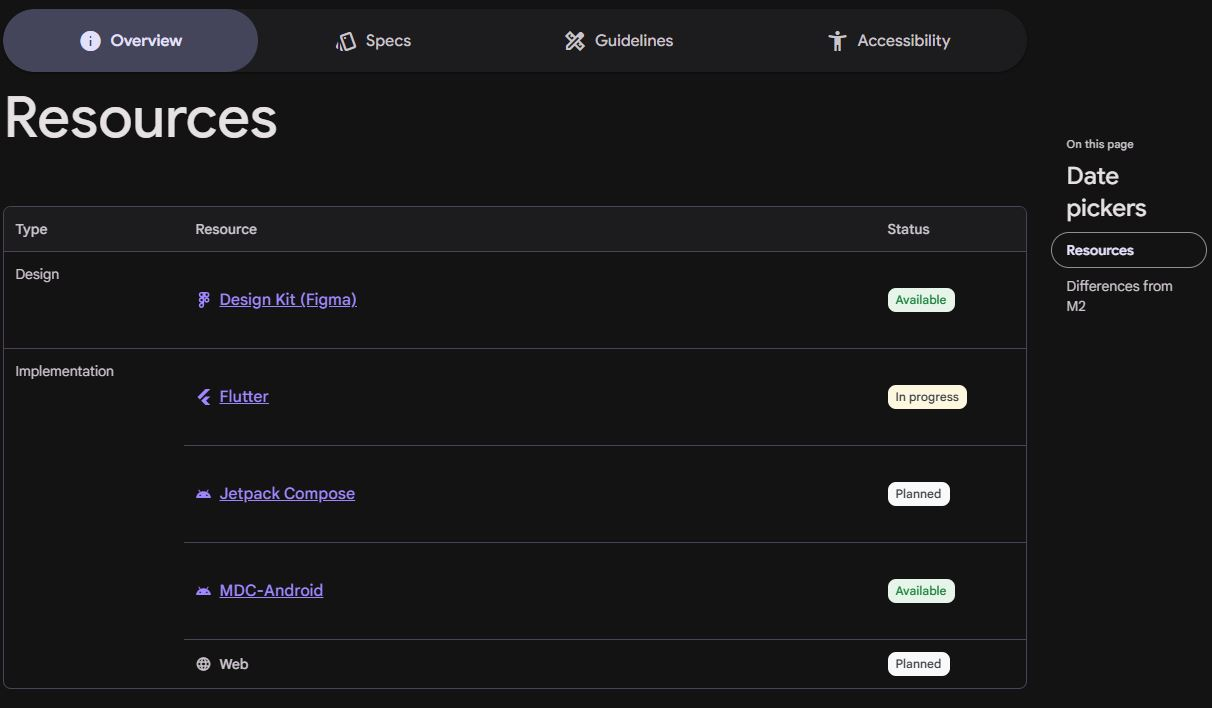
\includegraphics[width=0.75\textwidth]{figures/date_picker_status.JPG}
            \caption[Información oficial del elemento \textit{date picker}]
            {Información oficial del elemento \textit{date picker}. Imagen extraída de \cite{material_design_3_date_nodate}.}
            \label{figure:problemas:date_picker}
        \end{figure}
    
        \item \textbf{Dificultades notables para realizar pruebas}: los siguientes factores han complicado exponencialmente el proceso de pruebas, especialmente de cara a la automatización:
    
        \begin{itemize}
            \item El uso de \textit{Salud Conectada}, el cual aparece como una aplicación externa en versiones anteriores a la 14. Google no ha provisto aún una estrategia para realizar pruebas automáticas en aplicaciones que la integren.
            \item Ausencia de procedimientos oficiales o componentes para probar módulos que interactúan con el sistema operativo, tales como las notificaciones o la planificación de tareas.
            \item La implementación de los mecanismos de cambios de idioma, paletas de colores o modos.
        \end{itemize}
    
        \item \textbf{Ausencia de soporte para numerosas cuestiones}: las siguientes características implementadas en este proyecto disponen de un soporte muy limitado o inexistente, teniendo que acudir a librerías de terceros o afrontando numerosas dificultades técnicas:
            \begin{itemize}
                \item Cambio de idioma manual, detallado en la Sección \ref{section:implementacion:librerias_app}.
                \item Menús y diálogos de ajustes, detallado en la Sección \ref{section:implementacion:librerias_app}.
                \item Diseño de nuevos componentes gráficos, como el elemento de progreso circular.
                \item Elaboración de gráficas \gls{responsive} para móviles en posición apaisada.
                \item Modificación del eje X de las gráficas para mostrar el día de la semana y/o el día del año.
            \end{itemize}
        \item \textbf{Implementación de los cuestionarios}: debido a la naturaleza de los cuestionarios de la aplicación, fue particularmente complejo diseñar e implementar una arquitectura que permitiera implementar cuestionarios con diferentes tipos de preguntas (categóricas y numéricas), presencia o ausencia de mecanismos de puntuación, terminación temprana en el caso del cuestionario de suicidio, etc.
    \end{enumerate}

    % \section{Resultado: aplicación de Bienestar Emocional}

    % \todo[inline]{V: Cancelado por falta de tiempo.}

    % \todo[inline]{Falta en este capítulo una sección donde hagas un mini manual o una navegación por todas las pantallas de la app mostrando el resultado final}

    % \todo[inline]{Modo marketing, estilo libre}